\section{Approach Viability} \label{viability}

To verify the applicability of our detector and signature language, we tested the system by looking at several recent CVEs related to \ac{XSS}. We have three objectives: to verify that our signature language provides the necessary functionality to express an exploit and its patch, to test our detector against existing exploits, and to show that our signature language does not incur a high time overhead when writing a signature.

\subsection{Test methodology} \label{methodology}

Our evaluation focuses on recent CVEs related to WordPress
plugins. While this may seem restrictive, there are several reasons
why we targeted WordPress plugins:
\begin{itemize}
	\item WordPress powers 34.7\% of all websites according to a recent survey  \cite{w3stats} \cite{DBLP:journals/corr/abs-1801-01203}. The same study states that 30.3\% of the Alexa top 1000 sites use WordPress. Thus, we can be confident that our study results will hold true for the average user.
	\item WordPress plugins are very popular among developers (there are currently more than 55,000 plugins \cite{wpplugins}). Due to its user popularity, WordPress is also heavily analyzed by security experts. A search for WordPress CVEs on the Mitre CVE database \cite{cvemitre} gives 2310 results. Plugins, specifically, are an important part of this issue, 52\% of the vulnerabilities reported by WPScan are caused by WordPress plugins \cite{wpscan}.
	\item WordPress plugin code is accessible, so we can easily analyze both the client-side HTML, as well as the server-side code that generated it, which is helpful when writing signatures.
	\item Using one framework, we can install many different plugins for the version we want, reproduce attacks, and investigate the conditions under which they happen, without having to install additional software.
\end{itemize}

We looked at the 100 most recent WordPress \ac{XSS} CVEs, as of October 2018. We have chosen to use a CVE database, CVE Details \cite{cvedetails}, as opposed to other databases that include vulnerabilities or exploits, mainly because of reliability. We have been able to find hundreds of verified attacks on WordPress and its plugins using a CVE database, which also usually contain information on how to reproduce them. This provides the perfect platform to analyze \ac{XSS} attacks and decide whether they can be countered by our approach. 

For each CVE, we set up a Docker container with a clean installation of WordPress 5.2 and installed the vulnerable plugin's version. A few of the CVEs depended on the WordPress version as well, so we used the required WordPress version for those. Of the CVEs we looked at, only one of them occurred in WordPress core. We believe it would be harder to precisely sanitize injection points in WordPress core, as many of the plugins have very particular settings pages where the exploits occur, and the HTML is more identifiable. WordPress core, on the other hand, can be heavily altered by the use of themes and the user's own changes. However, as evidenced by our investigation, the vast majority of exploits occur in plugins.
 
 We then reproduced the exploit as described by the CVE. Finally, we analyzed the vulnerable page and wrote a signature to patch the exploit.

\subsection{Results}

\begin{table}[h!]
	\begin{center}
		\begin{tabular}{|c c|} 
			\hline
			Plugin & Installations\\ [1ex] 
			\hline
			WooCommerce  & 5+ million  \\  
			Duplicator & 1+ million \\  
			Loginizer & 900,000+ \\  
			WP Statistics & 500,000+ \\  
			Caldera Forms & 200,000+ \\   
			\hline
		\end{tabular}
		\caption{Most popular studied WordPress plugins}
		\label{table:1}
	\end{center}
\end{table}

Of the initial 100 CVEs, we were able to analyze 76 across 40 affected pages. We dropped 24 CVEs due to reproducibility issues: some of the descriptions did not include a PoC, making it difficult for us to reproduce; or, the plugin code was no longer available. In some cases, it had been removed from the WordPress repository due to "security issues", which emphasizes the importance of being able to defend against these attacks. This is not to say, however, that our detector would not work for such a CVE, as the author would have a better idea of how the exploit manifests itself, and would be in a better position to write a signature. The plugins we studied averaged 489,927 installations; \autoref{table:1} shows the number of installations for the 5 most popular studied plugins. For the vulnerabilities, 27 (35.5\%) could be exploited by an unauthenticated user; 56 (73.7\%) targeted a high-privilege user as the victim, 7 (9.2\%) had a low-privilege user as the victim, the rest affected users of all types.

Many of the studied CVEs included attacks for which there are known and widely deployed defenses. For example, many were cases of Reflected \ac{XSS}, where the URL revealed the existence of an attack, e.g:


$http://[path to WordPress]/wp-admin/admin.php?page=wps\_pages\_page\&page-uri=<script>alert("\ac{XSS}")</script>$

While Chrome's built-in \ac{XSS} auditor blocked this request, Firefox did not, and so we still wrote signatures for such attacks. In practice, we found several cases where even XSS auditor did not block the reflected XSS. We wrote 59 WordPress signatures in total, which got rid of the PoC exploit when sanitized with one of our three methods. Note that while PoCs are often the most simple form of an attack, our sanitization methods, and in particular DOMPurify, can get rid of complex injections as well. We were able to include several CVEs in some of them because they occurred in the same page and affected the same plugin. Overall, these signatures represent 71 (93.4\%) signed CVEs. The 5 we were not able to sign were due to lack of identifiers in the HTML, which would result in potentially large chunks of the document being replaced. For cases like these, the signature developer can weigh the trade-offs and decide whether the added cost is worth it.

After manual testing, the majority of the 71 signatures maintained the same layout and core functionality of the webpage. However, 12 signatures caused some elements to be rearranged, modifying the page's visual aspect. One caused a small part of the page to become unusable, due to the sanitization method used (a table showing user information was now rendered as blank). Most of the responsibility of maintaining functionality is left to the signature developer, being as precise as possible is key.

While our goal is to retain as much information of the page as possible after sanitization, we believe that even if a part of the page is now useless, this does not impact the user's experience as much, since most of these exploits occur in small sections of the HTML. A thorough study with regards to usability is out of scope for this work, but we provide some insight into false positives and false negatives in later sections, which is related to this issue.

\subsection{Generalizability} \label{generalizability}

To test the generalizability of our approach to other frameworks, we
analysed 5 additional CVEs, 2 related to Joomla!, 2 for LimeSurvey,
and 1 for Bolt CMS.  We chose Joomla! because it is another
popular \ac{CMS}. Unfortunately, we only found 2 CVEs
that we were able to reproduce, as the software for its extensions is
often not available. For fairness, we looked for the most recent CVEs
we could reproduce listed in the Exploit Database~\cite{exploitdb}, since
these have recorded \acp{PoC}. We carried out the same
procedure as with the WordPress CVEs, and were able to patch all of
the 5 exploits. This brought our CVE coverage rate up to 94.2\%.

\subsection{Signature writing times} \label{signature_times}

Figure ~\ref{fig:signature_times} shows a histogram of the time taken to write each of our signatures: this includes the time taken to check the HTML injection points, write the signature and debug it. We do not include the time taken to discover and carry out an exploit, as this is part of the CVE writing process. The median time is 3.89 minutes, and the standard deviation is 4.18 minutes. 72\% of signatures took less than 5 minutes to write. We believe this to be a reasonable amount of time for the security granted by our extension.

The signature which took the longest to write (25 minutes) corresponded to an exploit which had several injection points in the HTML, 12 exactly. Additionally, testing this signature proved more difficult than others, as some of the injections were a result of a script inserting elements in the DOM after the page had loaded. This caused the initial HTML to look innocuous, but with exploits still occurring after sanitization. As this script was part of the initial request, we eventually got to the root of the problem. We believe a more experienced exploit analyst might be able to detect this kind of behaviour more easily. Furthermore, having so many injection points in the HTML is cause for great complexity, and the writer can decide to block the page entirely, which would bring down the time taken.

Similarly, the second longest time taken (18 minutes) corresponded to an exploit which had 7 injection points, but each of these belonged to a part of the HTML with very generic element identifiers. Our language provides a means to overcome this, by being able to specify the element's "position": for example, if there are three <h3 class="title"> elements, in the HTML, and only one of them is an injection starting point, the writer can specify that the third one needs to be sanitized. The same happens for the ending points. As there were 7 of these such points, debugging took longer than for most of the other signatures. Again, this is a very complex case, and can be more prone to user error than other signatures, the writer might instead decide to block the page entirely.

Note that we have some signatures which cover several CVEs, as sometimes one page can have multiple CVEs associated with it. In particular, we had 6 of these, which had a median write time of 6.54 minutes. This means that the time per CVE is lower than the overall median of 3.89. Another source of increase timing is the more complicated case of listener type signatures, like ones for exploits caused by an XHR. We had 4 of these signatures, with a median write time of 9.86. As only a small number of these were present, we expect the time taken to write an average signature to be lower than the calculated total median.

\begin{figure}[h]
	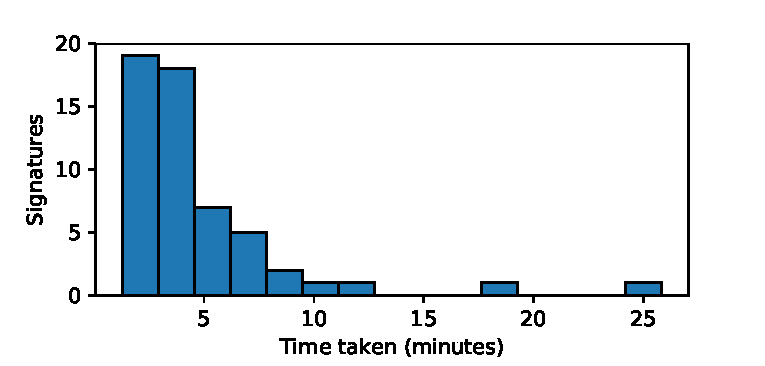
\includegraphics[scale=0.5]{results/signature_times_small.pdf}
	\caption{Histogram of time taken to write signatures.}
	\label{fig:signature_times}
\end{figure}


